\chapter{Dynamic Searchable Prefix Sum}
\label{chap:prefixsum}

In this chapter, the problem of dynamic searchable prefix sum is addressed with emphasis on achieving good practical performance. The problem is described along with some of its numerous applications. Related work in this area is then covered, followed by implementation details that are competitive with existing solutions. Finally, space requirements, time usage, and open problems are discussed.

The novel contributions of this chapter are: (i) an implementation of the dynamic searchable prefix sum based on Dietz's lazy synchronisation technique, achieving amortised $O(1)$ update time using SIMD (AVX-512) instructions; (ii) integration with the improved Fredman predecessor search from Chapter~\ref{chap:predecessor} to support constant-time \textit{select} operations; and (iii) a space analysis showing the data structure uses $n \log n + o(n)$ bits. Empirical evaluation of the proposed implementation is deliberately left for future work, as noted at the end of this chapter.
\section{Preliminaries}
The \textit{Prefix Sum} problem maintains an array $A$ with $n$ integers of \textit{m-bits} each with the following operations supported:
\begin{itemize}
    \item $sum(i)$ returns $\sum_{j=0} ^{i} A[i]$.
    \item $access(i)$ returns $A[i]$ such that $0 \leq i \leq n$.
    \item $update(i, \delta)$ modifies $A[i] = A[i] + \delta$ such that $0 \leq A[i] + \delta \leq 2^k - 1$.
\end{itemize}
A special case of this problem is when $m=1$, also known as the Dynamic Bit-Vector problem. This maintains a bit-vector of length $n$ that supports \textit{rank, select, and flip/update} operations \cite{Raman_2001}.

% Fredman \cite{Fredman_1982} established lower bounds for such problem, showing that under the cell probe model, the prefix sum problem cannot be solved faster than $\Omega(\log n/ \log \log n)$ per operation in the general case. However, in specialised memory architectures like the RAMBO model, it is possible to achieve constant time $O(1)$ solutions for both updates and queries \cite{Brodnik_2006}. Dietz \cite{Dietz_1989} supported \textit{sum} and \textit{update} optimally in $O(\log n/\log \log n)$ time for $m = \theta (\log n)$ using $\theta (n \log n)$ space. The work of Raman \cite{Raman_2001} improved on the space requirement to $mn + o(mn)$ bits for generalised $m = O(\log U)$ which is optimal within a lower-order term. 
% \par
\textbf{Naive approach}: Given $A$ of size $n$, we store $A$ plainly and answer \textit{sum} in $O(n)$ by scanning the array and \textit{update/access} in $O(1)$ with no extra space.
\begin{table}[H]
    \centering
    \begin{tabular}{|c|c|c|c|c|c|c|c|}\hline
         3 & 6 & 4 & 9 & 14 & 35 & 7 & 21 \\\hline 
         \multicolumn{1}{c}{0} & \multicolumn{1}{c}{1} & \multicolumn{1}{c}{2} & \multicolumn{1}{c}{3} & \multicolumn{1}{c}{4} & \multicolumn{1}{c}{5} & \multicolumn{1}{c}{6} & \multicolumn{1}{c}{7} \\
    \end{tabular}
    \caption{Array $A$ stored plainly to support \textit{increment/decrement} in $O(1)$}
    \label{tab:array-A-plain}
\end{table}
\begin{table}[H]
    \centering
    \begin{tabular}{|c|c|c|c|c|c|c|c|} \hline
         3 & 9 & 13 & 22 & 36 & 71 & 79 & 99 \\\hline 
         \multicolumn{1}{c}{0} & \multicolumn{1}{c}{1} & \multicolumn{1}{c}{2} & \multicolumn{1}{c}{3} & \multicolumn{1}{c}{4} & \multicolumn{1}{c}{5} & \multicolumn{1}{c}{6} & \multicolumn{1}{c}{7} \\
    \end{tabular}
    \caption{Array $B$ such that $B[i] = sum(i)$  to support \textit{sum} in $O(1)$}
    \label{tab:array-B-precomputed}
\end{table}
To support \textit{sum} in $O(1)$, we can use a pre-computed table $B$ of size $O(n \log n)$ such that $B[i] = sum(i)$, but \textit{update} will now be in $O(n)$. Both solutions are not optimal.
\par
\textbf{Better approach}: Using trees, we are able to achieve better results. A Segment-Tree \cite{Bentley_1977} used a balanced binary tree with the internal nodes storing the $sum$ of the elements of $A$ while the elements of $A$ are stored in the leaves. With a balanced binary-tree, the height is $\lceil \log n \rceil + 1$, and \textit{sum/update} operations can now be supported in $O(\log n)$ time. A Fenwick-tree \cite{Fenwick_1994} improves on the space usage by using an implicit tree to store $A$ using $n + 1$ machine words, but still needs $O(\log n)$ to answer the queries. This approach has been extended to \textit{b}-ary Segment-Tree with height of $\lceil \log_b n \rceil + 1$ allowing for queries to be answered in $O(\log_b n)$ and updates in $O(b\log_b n)$ \cite{Dietz_1989, Hon_2011, Patrascu_2006, Raman_2001}.
\begin{figure}[H]
\centering
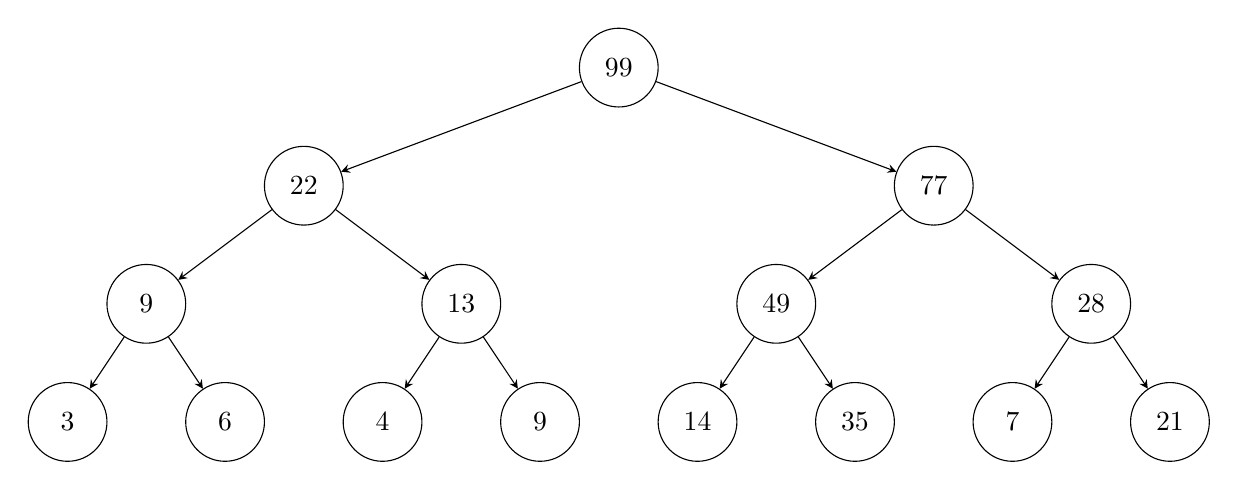
\begin{tikzpicture}[
  level 1/.style={sibling distance=8cm},
  level 2/.style={sibling distance=4cm},
  level 3/.style={sibling distance=2cm},
  edge from parent/.style={draw,-stealth},
  every node/.style={circle, draw, minimum size=1cm},
  sloped
  ]

  \node {99}
    child {node {22}
      child {node {9}
        child {node {3}}
        child {node {6}}
      }
      child {
        node {13}
        child {node {4}}
        child {node {9}}
      }
    }
    child {node {77}
      child {node {49}
        child {node {14}}
        child {node {35}}
      }
      child {node {28}
        child {node {7}}
        child {node {21}}
      }
    };

\end{tikzpicture}
\caption{Balanced binary tree storing prefix sums of $A$}
\label{fig:segment_tree}
\end{figure}
\FloatBarrier
\section{Related Work}
The foundational work by Fredman and Saks \cite{FREDMAN1993424} established a lower bound of $\Omega(\log n / \log w)$, which simplifies to $\Omega(\log n / \log \log n)$ for the common case where an integer fits within a word $w$. They also presented a trade-off $ \Omega(log n)$. Yao \cite{Yao_1985} independently found the same lower bound using a different approach for the amortised complexity of these operations. This indicates that any data structure supporting these operations must incur a logarithmic cost in the worst case. Hampapuram and Fredman \cite{Hampapuram_1998} demonstrated a $\Omega \log n$ lower bound for amortised complexity of the operations. They show the difficulty in reducing the complexity of these operations without compromising on performance in certain scenarios. Dietz \cite{Dietz_1989} introduced a data structure meeting Fredman and Saks' lower bound for both operations, requiring $\delta = O(\log \log n)$, handling $b = O(\log^{\varepsilon} n)$ elements in constant time, and utilising a Segment-Tree with branching factor $b$. This solution was enhanced by Raman \cite{Raman_2001} and Hon \cite{Hon_2011}, though it necessitated large universal tables that scaled poorly with $\delta$ and $b$.\par
Pătraşcu \cite{Patrascu_2006} further refined these lower bounds and trade-offs, presenting a parametric lower bound in terms of $w$ and $\delta$. They distinguished between cases where $\delta = \Omega(w)$ and $\delta = o(w)$. For $\delta = \Omega(w)$, they identified the logarithmic bound $\Omega(\log n)$ and two symmetrical trade-off lower bounds of $\Omega(\log n)$, confirming the optimal results of Segment-Tree and Fenwick-Tree structures. For $\delta = o(w)$, they found a trade-off lower bound of $\Omega(\log n)$, leading to $\Omega(\log n / \log(w/\delta))$. They proposed a data structure achieving $O(\log n / \log(w/\delta))$, optimal for this lower bound. Their approach involved supporting operations in constant time on b elements, building a Segment-Tree with branching factor b, and packing array $C$ in $w$ bits for constant-time manipulation, feasible as long as $b = O(w/(\delta + \log w))$.\par
Extensive work from theoretical point of view has been studied on this problem \cite{Bille_2017, Bille_2018, Chan_2010, Fredman_1982, Hampapuram_1998, Hon_2011, Patrascu_2006, Yao_1985}  due to its promising applications in areas of coding, databases, and creating dynamic data structures. Pibiri \cite{Pibiri_2020}  explored various c++ implementation of prefix sum data structure and their optimisations.
\FloatBarrier
\section{Searchable Prefix Sum}
The \textit{Searchable Prefix Sum} problem maintains an array $A$ of $n$ positive integers that supports all the operations in the \textit{static prefix sum} with the additional operation below:
\begin{itemize}
    \item select(i): returns the index of the successor of $i$ in $A$.
\end{itemize}
Raman \cite{Raman_2001} built on \cite{Dietz_1989} to propose a data structure that supports all operations in $O(\log n / \log \log n)$ time while using \textit{kn + o(kn)} bits. They started by solving the problem in small sets of integers that supports all operations in constant time.\par
\textbf{Lemma 1:} On a RAM model, searchable partial sum problem on a sequence of $m = w^\epsilon$ for a fixed $\epsilon$ such that $0 \leq \epsilon \leq 1$ on set $S$ and $k = |S|$ and $k \leq w$, the data structure stores $S$ using $O(mw)$ bits and supports operations in $O(1)$ using $O(2^{\epsilon^1 w})$\par
\textit{Proof:} Let $S$ be the set of elements that for which their partial sums are to be calculated. Let $B$ be another table such that $B[i] = \sum_{j=0}^{i} A[j]$. Using \cite{Dietz_1989}, we can let $B$ to go out of \textit{sync}, where not all updates are immediately effected on $B$. Otherwise, \textit{updates} will be in $O(m)$. So, for every $m$ updates, we then refresh $B$ to bring it up to date. This brings the \textit{update} operation on $B$ to amortised $O(1)$.\par
For queries, we maintain a buffer array $C$ on size $n$ to track the out of sync updates. When we want to update $B[i]$ by $\delta$, we instead update $C[i] = C[i] + \delta$. Since $|C[i]| \leq m\delta = w^{O(1)}$, $C$ uses $O(m\log w)$ bits. Dietz \cite{Dietz_1989} supports \textit{sum(i)} by accessing $B[i] + C[i]$ where $C$ is indexed into a pre-computed table.Using \textit{Q-heap} proposed by Fredman \cite{Fredman_1982}, Raman showed how to support \textit{search(i)} in $O(1)$. \par
\textbf{Theorem 1:} For $0 \leq M \leq 2^w$, we can support \textit{insert, delete, update, predecessor and successor} operations in $O(1)$ for $|S| = \log M^{1/4}$. The \textit{successor(x)} is the largest $s \in S$ such that $y \geq x$, while the \textit{predecessor(x)} is the largest $s \in S$ such that $y \leq x$. There is need for a pre-computed table of size $O(M)$ to achieve this. 
\par More information on this can be found in \cite{Raman_2001}.
\FloatBarrier
\section{Dynamic Searchable Prefix Sum}
This section presents an implementation of a variation of Dietz's \cite{Dietz_1989} data structure using Single-Instruction-Multiple-Data instructions on $A$ where $|A|$ is a small set of integers. The main concern is how to maintain and update $B$ in amortised $O(1)$, and support \textit{select} in $O(1)$. Simple yet efficient strategies are presented for maintaining $B$ and $C$ using a combination of arrays and SIMD registers, combined with the improved data structure proposed in Chapter \ref{improved-fredman} that allows constant time \textit{select}.\par
The proposed data structure supports the following operations:
\begin{itemize}
    \item $sum(i):$ return $\sum_{j=0}^{i} A[j]$
    \item $increment(i):$ updates $A[i] = A[i] + 1$
    \item $select(j):$ returns the smallest $i$ such that $sum(i) \geq j$
\end{itemize}
The data structure supports \textit{sum and select} operations in $O(1)$ while \textit{increment} operates in amortised $O(1)$. Given $A$ of size $n$, the prefix sum array $B[i] = \sum_{j=0}^{i} A[j]$ is computed. A buffer array $C$ of size $O(w^{O(1)})$ is maintained that can be updated in $O(1)$. The value $m = \max\{B[i] - B[i+1]\}$ is determined to be the largest gap between the elements in $B$, and a counter tracks the number of updates so far. The idea is to refresh $B$ to bring it up to date with $C$ after every $counter = m$ updates on $C$. A mask $m_c$ \textit{p} of size $w$ is calculated that sets $p_i$ to $1$ if it is a branching bit in $B$; this mask is used to compress values in $B$. An array $D$ of size $O(w^{O(1)})$ is maintained that stores the compressed values of $B$ such that $D[i] = compress(B[i], m_c)$, and whenever $B$ is refreshed, $D$ is reconstructed. It should be noted that $C$ and $D$ can store $n$ items.\par
Using SIMD registers and builtin instructions, $C$ and $D$ can be stored in AVX-512 registers\footnote{\url{https://www.intel.com/content/www/us/en/docs/intrinsics-guide/index.html\#techs=AVX\_512}} allowing up to 512 bits to be processed at the same time. To compress $B$, we use the standard \text{\_pext\_u64}\footnote{\url{https://www.intel.com/content/www/us/en/docs/intrinsics-guide/index.html\#text=pext\&ig\_expand=5088}} to extract the \textit{most significant bits} from $B$ in $O(1)$. It is known that $C$ and $D$ can support operations such as \textit{addition, subtraction, multiplication, access, etc.} in constant time as well.\par
\begin{table}[H]
\centering
    \begin{tabular}{|c|c|c|c|c|c|c|c|}
            \hline
             14 & 5 & 6 & 8 & 3 & 1 & 12 & 1 \\
            \hline
        \end{tabular}
    \caption{Array $A$ with original sequence}
    \label{tab:array-A-original}
\end{table}
\begin{table}[H]
\centering
    \begin{tabular}{|c|c|c|c|c|c|c|c|}
            \hline
             14 & 19 & 25 & 33 & 36 & 37 & 49 & 50 \\
            \hline
        \end{tabular}
    \caption{Array $B$ with possibly out of \textit{sync} prefix sums}
    \label{tab:array-B-out-of-sync}
\end{table}
\begin{table}[H]
\centering
        \begin{tabular}{|c|c|c|c|c|c|c|c|}
            \hline
            0 & 0 & 2 & 1 & 1& 1& 4 & 3\\
            \hline
        \end{tabular}
    \caption{SIMD Array $C$ with all the recent updates}
    \label{tab:array-C-updates}
\end{table}
\begin{table}[H]
\centering
        \begin{tabular}{|c|c|c|c|c|c|c|c|}
            \hline
            14 & 19 & 27 & 37 & 40& 42& 58 & 62\\
            \hline
        \end{tabular}
    \caption{Array $B$ after $m=12$ updates is now refreshed with $C$}
    \label{tab:array-B-refreshed}
\end{table}

% \begin{table}[H]
% \centering
%         \begin{tabular}{|c|c|c|c|c|c|c|c|}
%             \hline
%             0 & 0 & 2 & 4 & 4& 4& 4 & 9\\
%             \hline
%         \end{tabular}
%     \caption{SIMD Array $D$ with compressed values of $B$}
%     \label{tab:my_label}
% \end{table}
\FloatBarrier
\section{Operations}
\textbf{\textit{sum(i)}}: To support $sum(i)$, we simply return $B[i] + \sum C[i]$. This may appear to be slower than normal, but $C$ is expected to fit into very fast memory and can be computed in constant time. So the impact is negligible.\par
\textbf{\textit{access(i)}}: To support $access(i)$, we simply return $sum(i) - sum(i-1)$.\par
\textbf{\textit{increment(i)}}: $C$ is simply updated by generating an update $mask$ starting with all elements in the mask to be zero, and then set $C[i]$ to 1 for $0 \leq i < n$. Adding the $mask$ and $C$ is a simple SIMD addition in $O(1)$. The update counter $counter$ is then incremented. If $counter = m$, $B$ is refreshed by setting $B[i] = B[i] + \sum C[i]$ for $0 \leq i < n$. $B$ is also compressed into $D$ as described earlier, then recompute $m$ and reset $counter$.\par
\textbf{\textit{select(j)}}: As $D$ stores the compressed values of $B$, we can equally compress $j$. Then search for $j$ in $D$ using SIMD instructions as described in Section \ref{improved-fredman}. This is also done in $O(1)$.\par
It is clear that for space usage, $B$ can be stored using $n\log n$ bits. Only $O(w^{O(1)}$ to store $C$ and $D$, which is $o(n)$. This data structure uses $n\log n + o(n)$ bits.
\FloatBarrier
\section{Optimisations}
The \textit{access(i)} and \textit{update} operations can be optimised further. During updates, instead of updating a single element in $C$, a mask can be generated that sets $mask[i]$ for all $0 \leq i < n$. Then $mask[j] = 1$ is set for all $i \leq j < n$. This way, $C$ is maintained as a prefix sum as well. When refreshing, only $B[i] = B[i] + C[i]$ needs to be set. Likewise, when accessing elements or performing sum operations, $C$ can be directly accessed without having to sum up the values in $C$.

\FloatBarrier
\section{Chapter Summary}

This chapter addressed the problem of dynamic searchable prefix sum, which maintains an array of integers supporting sum queries, updates, and search operations. The following contributions were presented:

\begin{itemize}
    \item A review of the theoretical foundations, including Fredman and Saks'~\cite{FREDMAN1993424} lower bound of $\Omega(\log n / \log \log n)$ for prefix sum operations, and the optimal solutions proposed by Dietz~\cite{Dietz_1989} and Raman~\cite{Raman_2001}.

    \item An implementation approach based on Dietz's lazy synchronisation technique, where a buffer array $C$ accumulates updates before periodically refreshing the main prefix sum array $B$. This achieves amortised $O(1)$ update time.

    \item The application of SIMD instructions (AVX-512) to store and manipulate the buffer arrays $C$ and $D$, enabling constant-time operations on small integer sets.

    \item Integration with the improved Fredman predecessor search technique from Chapter~\ref{chap:predecessor} to support constant-time \textit{select} operations by maintaining compressed representations of prefix sums.

    \item Space analysis showing that the data structure uses $n \log n + o(n)$ bits, with the $o(n)$ overhead coming from the SIMD-compatible buffer structures.
\end{itemize}

The proposed implementation builds upon the data structures developed in earlier chapters, demonstrating how extensible arrays (Chapter~\ref{chap:extensible}) and fast predecessor search (Chapter~\ref{chap:predecessor}) can be composed to create efficient dynamic searchable prefix sum structures.

\textbf{Note on Empirical Evaluation.} A full empirical evaluation of the dynamic searchable prefix sum implementation is deliberately deferred to future work. A meaningful comparison would require complete integration of the extensible array (Chapter~\ref{chap:extensible}) and predecessor search (Chapter~\ref{chap:predecessor}) components with AVX-512 hardware support. Future work will include benchmarking against existing solutions such as Pibiri's~\cite{Pibiri_2020} C++ implementations, evaluating performance across varying array sizes and update frequencies, and measuring the practical overhead of the lazy synchronisation strategy.
